% !TEX TS–program = pdflatexmk

\documentclass[lucida,biblatex]{sp} % use if you have the Lucida LaTeX fonts
%\documentclass{sp}          % default: uses Times font
\usepackage{textcomp}
\usepackage{algorithm}
\usepackage{algpseudocode}
\usepackage{tikz}
\usepackage{tikz-dependency}
\usepackage{gb4e}
\usepackage{amssymb}
\usepackage{pifont}
\usepackage{tipa}
\usetikzlibrary{fit,positioning}
\usepackage{setspace}
\usepackage{color}
\usepackage{bbm}
\usepackage{enumitem}
\usepackage{mathrsfs}  
\usepackage{bbm}


\addbibresource{references.bib}

\usepackage[utf8]{inputenc}

%\linespread{2}


%tables
\usepackage{tabularx}
\usepackage{array}
\usepackage{booktabs}
\usepackage{multirow}
\newcolumntype{L}[1]{>{\raggedright\let\newline\\\arraybackslash\hspace{0pt}}m{#1}}
\newcolumntype{C}[1]{>{\centering\let\newline\\\arraybackslash\hspace{0pt}}m{#1}}
\newcolumntype{R}[1]{>{\raggedleft\let\newline\\\arraybackslash\hspace{0pt}}m{#1}}
\newcommand{\possessivecite}[1]{\textciteauthor{#1}'s (\textciteyear{#1})}

\newcounter{excounter}

%=====================================================================
%========================= preamble material =========================

% Metadata for the PDF output. ASCII-only!
\pdfauthor{Sebastian Schuster and Judith Degen}
\pdftitle{Listener adaptation to speaker variation in use of uncertainty expressions}
%\pdfkeywords{Full keyword list}

% Optional short title inside square brackets, for the running headers.
% If no short title is given, no title appears in the headers.
\title{Listener adaptation to speaker variation in use of uncertainty expressions}

% Optional short author inside square brackets, for the running headers.
% If no short author is given, no authors print in the headers.
\author{% As many authors as you like, each separated by \AND.
  \spauthor{Sebastian Schuster and Judith Degen\\ \today}
}

%=====================================================================

\begin{document}

%=====================================================================
%============================ frontmatter ============================

\maketitle

%\begin{abstract}

%\end{abstract}

%\begin{keywords}
%  Keywords (special formatting is fine)
%\end{keywords}

%=====================================================================
%============================ article text ===========================

\section{Introduction}

We are studying a) whether speakers show variation in their use of expressions of uncertainty (e.g., \textit{might} or \textit{looks like}) and b) whether listeners adapt to different uses of expressions of uncertainty by different speakers through experiments and computational modeling.

\section{Experiments}

\subsection{Pre-test experiment}

The first series of experiments was intended to evaluate whether there was variation in the use of expressions of uncertainty. We asked participants to rate how likely they thought it was that a speaker would use different expressions of uncertainty to describe the possibility of an event happening. More concretely, participants were presented with scenes in which they saw an adult and a child next to a gumball machine with orange and blue gumballs. In each scene, the child uttered \textit{``I want a blue one''} or  \textit{``I want an orange one''} (randomized across participants, except in the first condition in which this was also randomized within participants). Participants were instructed that the adult can see the contents of the gumball machine but the child cannot and they were asked to indicate how likely they think the speaker is to use the two utterances that are presented below the scene, or something else, by distributing 100 points using three sliders. Within each of the 15 conditions, participants always saw two of the following six utterances:

\begin{itemize}
\item You'll get a blue/orange one (\textsc{bare})
\item You might get a blue/orange one (\textsc{might})
\item You'll probably get a blue/orange one (\textsc{probably})
\item I think you'll get a blue/orange one (\textsc{think})
\item It looks like you'll get a blue/orange one (\textsc{looks like})
\item You could get a blue/orange one (\textsc{could})
\end{itemize}

This was a between-subjects design with 20 participants per condition and each participant saw trials from only one condition, i.e., each participant saw the same two utterances in all trials. Within each condition, we manipulated the percentage of blue gumballs. Each participant saw 3 trials for each of the following percentages: \\ 0\%, 10\%, 25\%, 40\%, 50\%, 60\%, 75\%, 90\%, 100\%.

\begin{center}
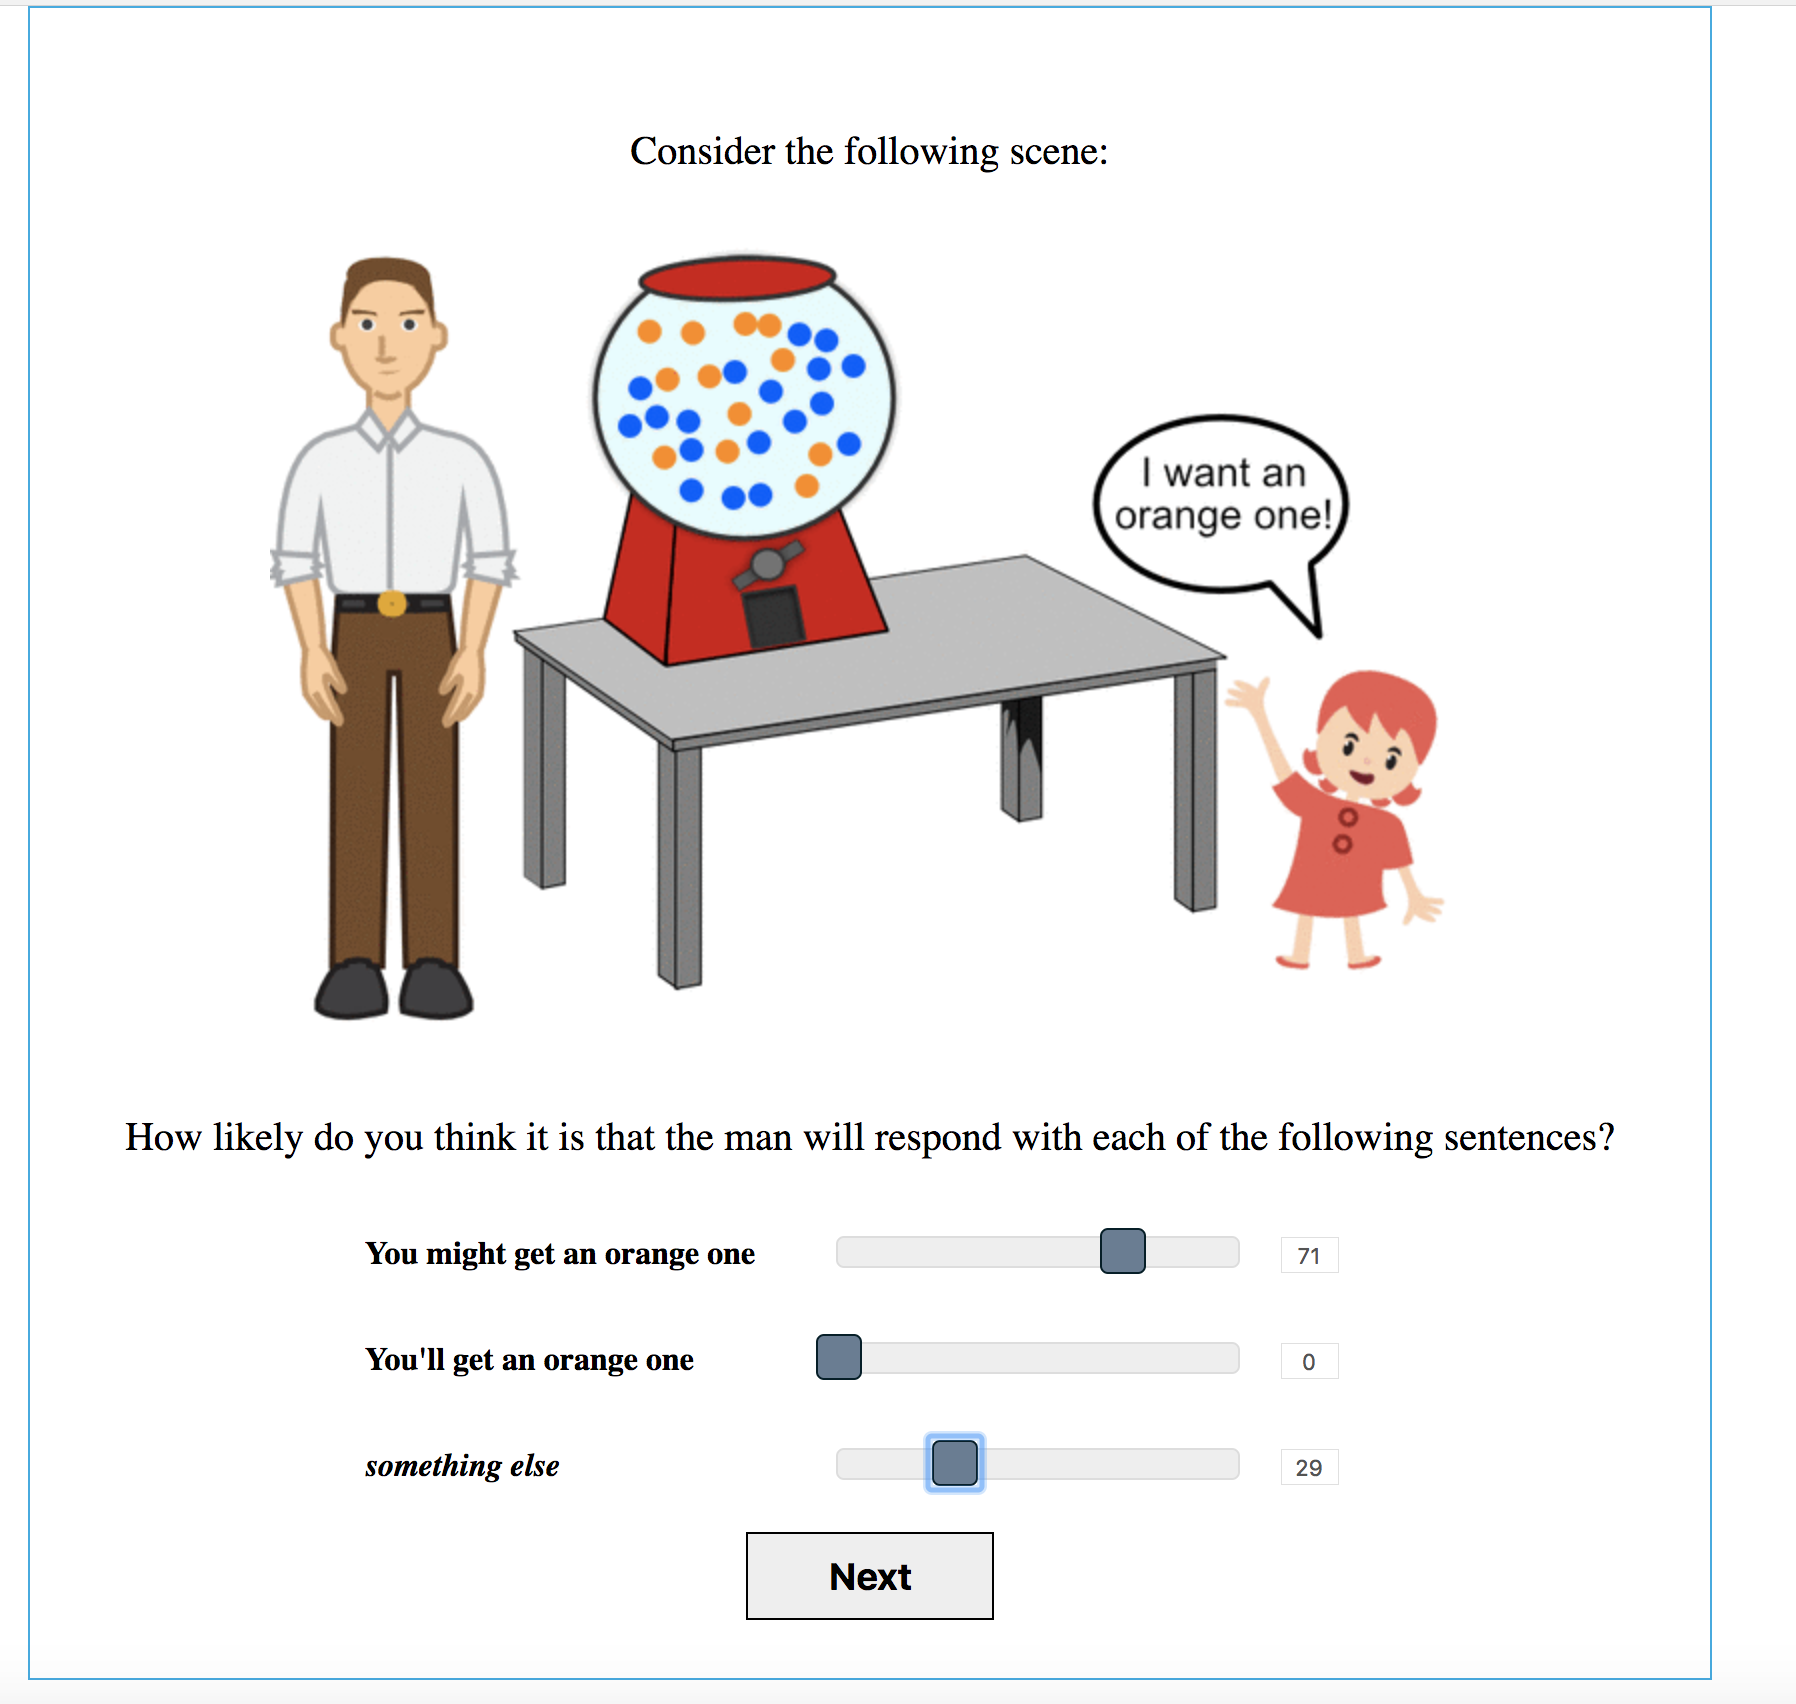
\includegraphics[width=\textwidth]{figures/pre-test-example-trial.png} 
\vspace{2em}
\end{center}

\subsubsection{Results}

The following plot shows the results for the might-probably condition in which participants always saw the two utterances \textit{You might get a blue/orange one} and  \textit{You'll probably get a blue/orange one}.\footnote{See \url{https://github.com/sebschu/adaptation/blob/master/experiments/0_pre_test/analysis/results.html} for results from all 15 conditions.} 

\begin{center}
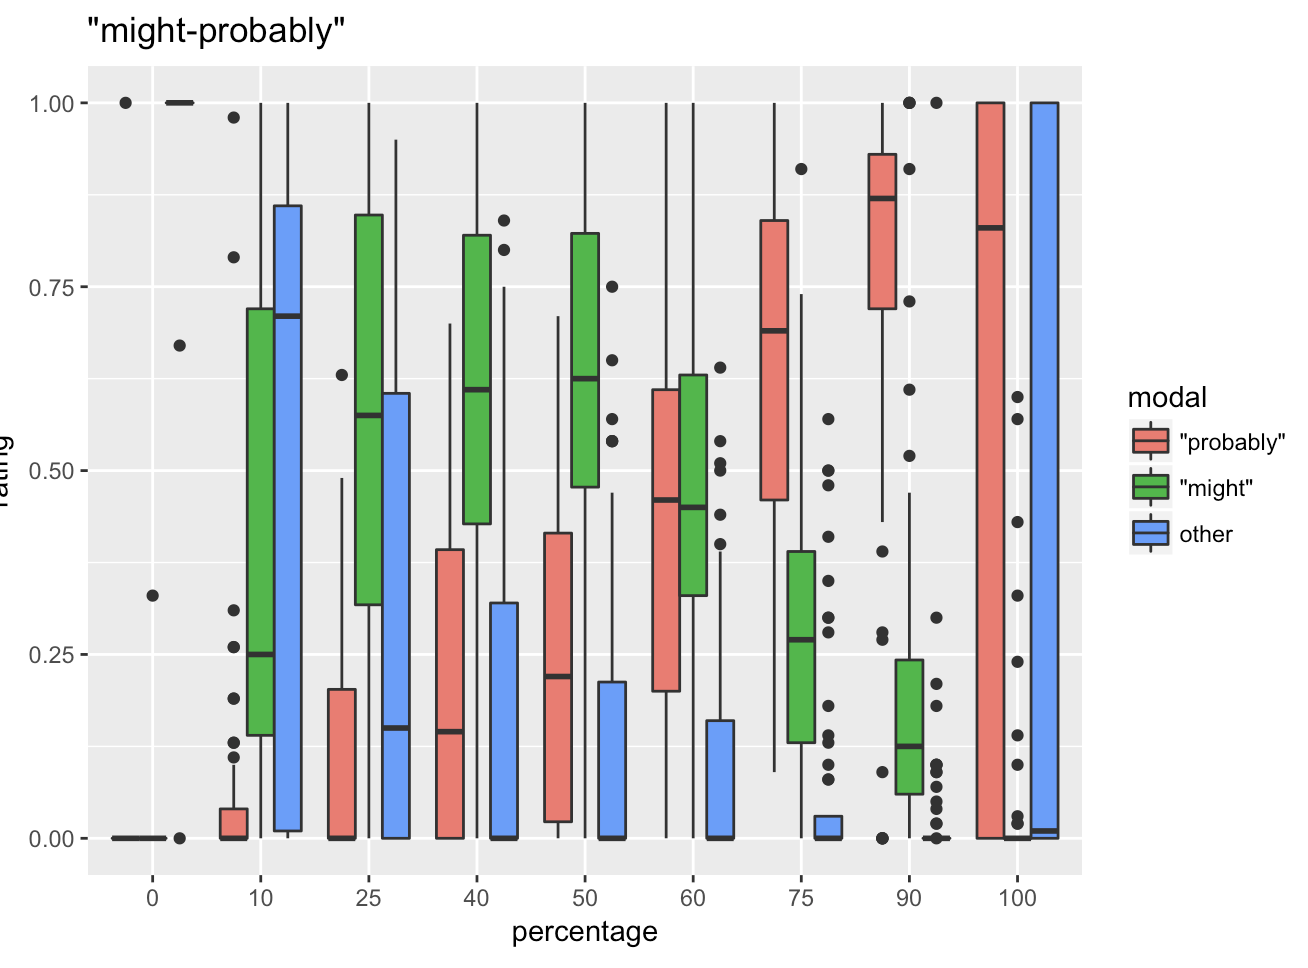
\includegraphics[width=\textwidth]{figures/pre-test-results.png}
\vspace{2em}
\end{center}

As this plot shows, there is considerable variation in the use of these two expressions when there is a 60\% chance of getting a blue gumball and for this percentage of blue gumballs, some participants rate \textit{might} higher than \textit{probably} and vice versa. We therefore chose this condition to study whether listeners adapt their speaker expectations after being exposed to a speaker for some time.


\subsection{Adaptation experiment}

For the adaptation experiment, we only considered the condition in which speakers have to choose between \textit{might}, \textit{probably}, and other. In this experiment, participants first watched in total 20 scenes in which they again saw a child and a gumball machine with different percentages of blue gumballs. Instead of the cartoon adult, participants watched a short video in which in each trial a man or a woman (speaker gender was randomized across participants) spoke one of the following three utterances:

\begin{itemize}
\item You'll get a blue/orange one (\textsc{bare})
\item You might get a blue/orange one (\textsc{might})
\item You'll probably get a blue/orange one (\textsc{probably})
\end{itemize}

The number of times participants heard these utterances and the types of scenes (i.e., the percentages of blue gumballs) varied across two conditions. Participants in the \textbf{probably-biased} condition, saw 5 \textsc{bare} filler trials with 100\% blue gumballs; 5 \textsc{might} filler trials with 25\% blue gumballs; and 10 critical \textsc{probably} trials with 60\% blue gumballs. Participants in the \textbf{might-biased} condition, saw  5 \textsc{bare} filler trials with 100\% blue gumballs; 5 \textsc{probably} filler trials with 90\% blue gumballs; and 10 critical \textsc{might} trials with 60\% blue gumballs. The filler trials always corresponded to roughly the percentages of blue gumballs for which participants rated the three utterances to be most likely in order to convey that this is a reasonable speaker (following the design by Yildirim et al. (2016)).

After the exposure phase, participants did the same rating task as in the pre-test experiment. There were 40 participants in each condition.

\subsubsection{Results}

The following plots shows the aggregated post-exposure ratings in the two conditions.

\begin{center}
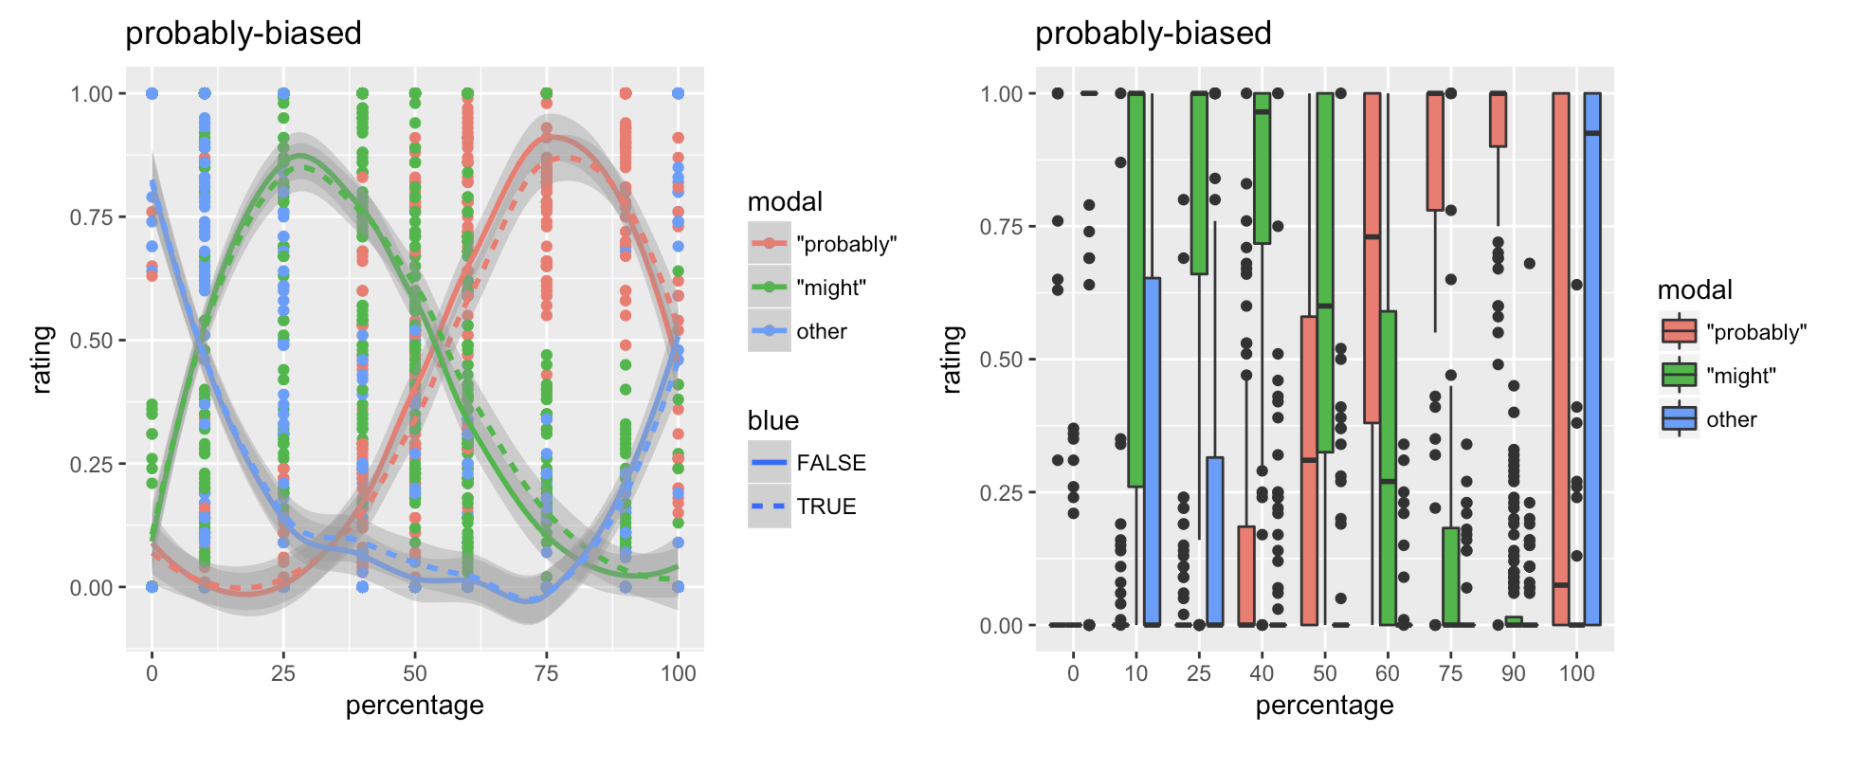
\includegraphics[width=\textwidth]{figures/adaptation-probably-biased-results.png}

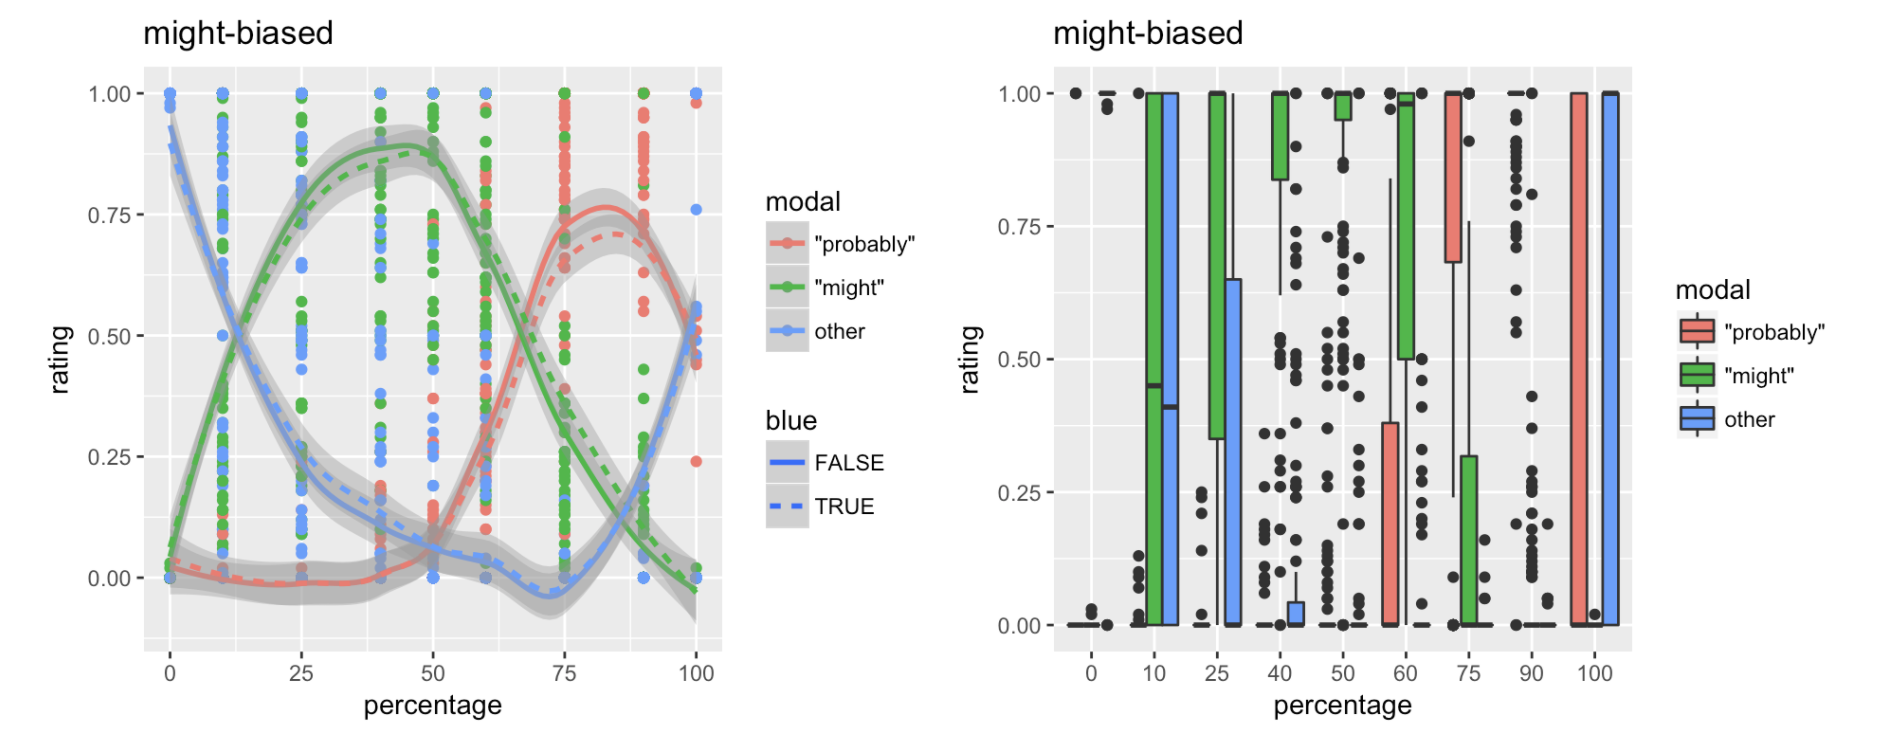
\includegraphics[width=\textwidth]{figures/adaptation-might-biased-results.png}
\vspace{2em}
\end{center}

As these plots show, participants gave high ratings for \textit{probably} for a larger range of event probabilities in the \textit{probably-biased} condition than participants did in the \textit{might-biased} condition; and participants gave high ratings for \textit{might} for a larger range of event probabilities in the \textit{might-biased} condition than participants did in the \textit{probably-biased} condition. This suggests that participants actually picked up on the different uses of these expressions and adjusted their speaker expectations accordingly.

We also performed a similar analysis as Yilldirim et al. (2016) and compared the differences in the area under the curve (AUC) between the \textit{might} and the \textit{probably} curve across the two conditions and found that the differences in AUC are significantly different across the two conditions ($t(59) = 4.9821$, $p < 0.00001$). 

\section{Models}

While the results of the two experiments suggest that there is considerable variation in the use of uncertainty expressions and that listeners can adapt their speaker expectations after listening to a speaker several times, the experimental results do not explain the adaptation process. We therefore also attempt to model participant behavior using a Bayesian cognitive model.

\subsection{Pre-test experiment}

\subsubsection{Model}

We model the process that leads to the experimental results in the pre-test experiment as a speaker model ($S_1$) in the Rational Speech Acts framework \citep{RSA}. We assume that participants take the role of a generic speaker but given that they reason about a non-specific speaker, participants have some uncertainty about the speaker's language use.

Within the RSA framework, a pragmatic speaker reasons about a literal listener ($L_0$). In the context of our experiment, we define the following literal listener in a similar vain as Lassiter and Goodman (2015) and Herbstritt and Franke (2017). 
$$L_0(\phi \mid u; \theta) \propto P(\phi) \left( {0.95} \times \mathbbm{1}[\phi > \theta_{u}] + 0.05 * P_{uniform}(\phi; 0,1) \right)$$

The literal listener tries to infer the probability $\phi$ of an event happening (in our case, the probability of getting a blue gumball) from an utterance with an uncertainty expression $u$. We assume that for each uncertainty expression, there is some threshold $\theta_u$ such that $u$ is semantically felicitous if  $\phi$ is above this threshold. We assume that the prior $P(\phi)$ is uniform. Given that we are dealing with noisy experimental data, we also include a noise term of the form $0.05 * P_{uniform}(\phi; 0,1)$, which allows for random inferences in 5\% of the cases. 

\vspace{1em}

\textbf{Q:} Is this a reasonable way to model noise?

\vspace{1em}


We assume that each uncertainty expression has its own threshold, except for the negated version of the bare statement, which we assume to be true if $\phi$ is less than $1-\theta_{bare}$ (Herbstritt and Franke, 2017).

Given this literal listener, a pragmatic speaker $S_1$, tries to maximize the listener's utility when choosing an utterance to convey the probability $\phi$. We assume that a speaker chooses among the 6 utterances that were used across the 15 conditions and the the negated version of the bare statement, i.e., \textit{"You won't get a blue one"}.
$$S_1( u \mid \phi, condition; \theta ) \propto exp \left(\lambda \left( \log P_L(\phi \mid u; \theta) - c(u, condition) \right) \right) $$

Following the vanilla RSA model, we define the utility as the negative surprisal subtracted by the cost of the utterance. Given our experimental setting in which we ask participants to choose between two given utterances and \textit{other}, we use the following cost function, which depends on the experimental condition.
$$
c(u, condition) = 
     \begin{cases}
       0 &\quad\text{if } u  \text{ is one of the utterances in } condition\\
       c_{u} &\quad\text{otherwise} \\
     \end{cases}
$$

The motivation here is that participants will be primed to use the two given utterances, which is reflected in the lower cost.

The $S_1$ model that we presented here is still parameterized by a set of thresholds $\theta$. Considering the variation in use of uncertainty expressions, participants seem to show uncertainty about how a generic speaker would set $\theta$ for the individual uncertainty expressions. We therefore assume that participants come with a prior over reasonable thresholds and given that they are asked to reason about an unknown speaker, they marginalize over this prior to derive the distribution over utterances, which results in the following revised speaker model.

$$P_S(u \mid \phi, condition) \propto \int P(\theta) exp\left(\lambda  \left(\log P_L(\phi \mid u; \theta) - c(u, condition)\right)\right) d\theta $$

\subsubsection{Parameter estimation}

Our model has 14 parameters, namely 6 prior distributions over thresholds $P(\theta_u)$, 7 cost terms $c_u$, and the rationality parameter $\alpha$, which we all estimate from the experimental data. For the prior distributions $P(\theta_u)$, we assume that these follow a beta distribution parametrized by $\alpha_u$ and $\beta_u$ (Qing (2014) made similar assumptions for modeling the use of \textit{some} and \textit{many}). There are two main reasons for choosing a beta distribution: First, its range is from 0 to 1, and given that $\theta$ defines a threshold parameter for a probability, this matches exactly the reasonable interval for the thresholds. Second, the beta distribution can take very different shapes and therefore we are not making the assumption that all of the prior distributions over thresholds have a similar shape.

To facilitate computations, we discretize our speaker and listener model as well as the priors over thresholds and infer these distributions by enumerating all possibilities. To estimate the model parameters, we run MCMC with 8,000 burn-in samples and 12,000 samples.\footnote{Note that this does not seem to be enough samples yet as 3 different runs still lead to varying results and don't pass the criterion by Gelman and Rubin (1992). I'm currently running the model again with 100,000 samples, which will hopefully be enough for stable parameter estimates.} 

We sample parameters from the following distributions.

$$\alpha_u, \beta_u \sim Uniform(0,30)$$
$$c_u\sim Uniform(0,5)$$
$$\lambda \sim Uniform(0.1,3)$$

We then estimate the parameters by computing the distributions over parameters given the experimental data across all 15 conditions $\mathscr{D}$.

\begin{align*}
P(\alpha,\beta, c, \lambda \mid \mathscr{D}) &\propto P(\alpha, \beta, c, \lambda) P(\mathscr{D} \mid \alpha,\beta, c, \lambda) \\
&= P(\alpha, \beta, c, \lambda) \prod_{d \in \mathscr{D}} P_S(u_d \mid \phi_d, condition_d; \alpha, \beta, c, \lambda)
\end{align*}

Note that for each probability $\phi$, participants provided a distribution over utterances and not actual samples of utterances given $\phi$. For each trial in which a participant provided a distribution over utterances, we therefore sampled 10 utterances from this distribution and combined all of these samples to form the data $\mathscr{D}$ from which we estimated the parameters of our model.

For each parameter, we take the median of the 12,000 MCMC samples and use these parameter estimates for making model predictions.


\subsubsection{Model predictions}

The following plots show the experimental results (left) and the model predictions (middle) for several (representative) conditions.\footnote{See \url{https://github.com/sebschu/adaptation/blob/master/models/1_threshold_modals/prediction_model.html} for results for all 15 conditions.}

\begin{center}
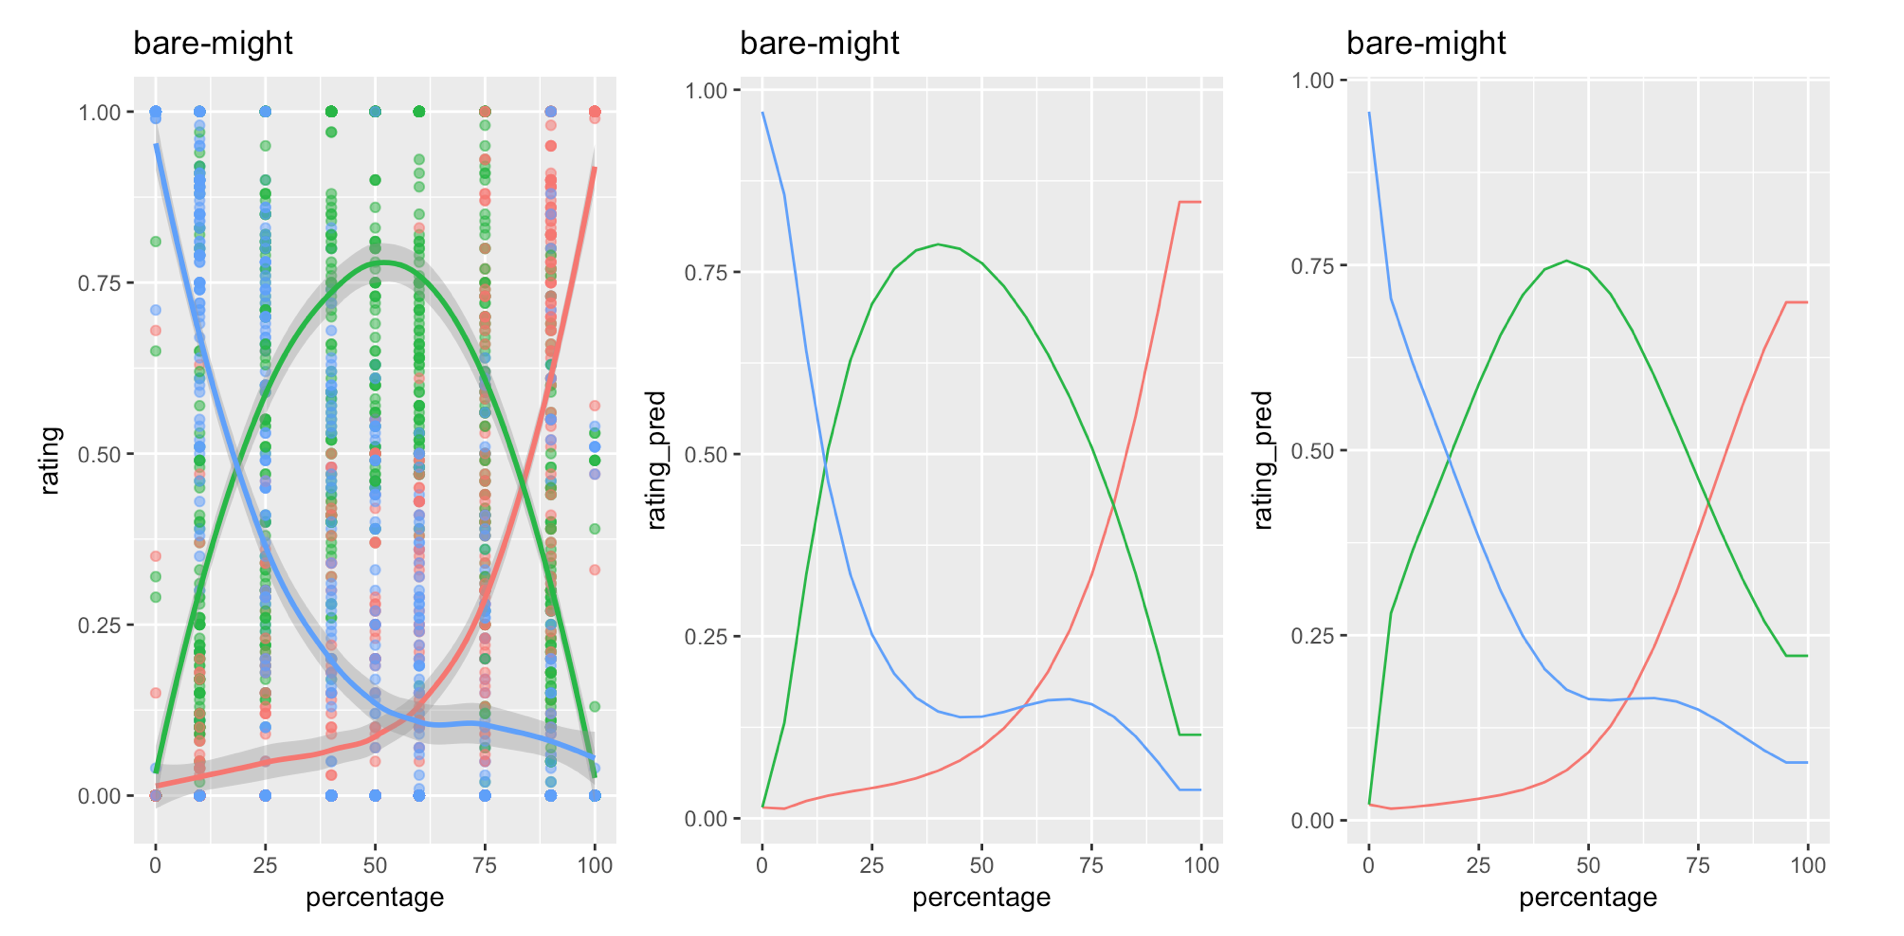
\includegraphics[width=\textwidth]{figures/bare-might-predictions.png} \\
bare (red) - might (green) condition

\vspace{2em}

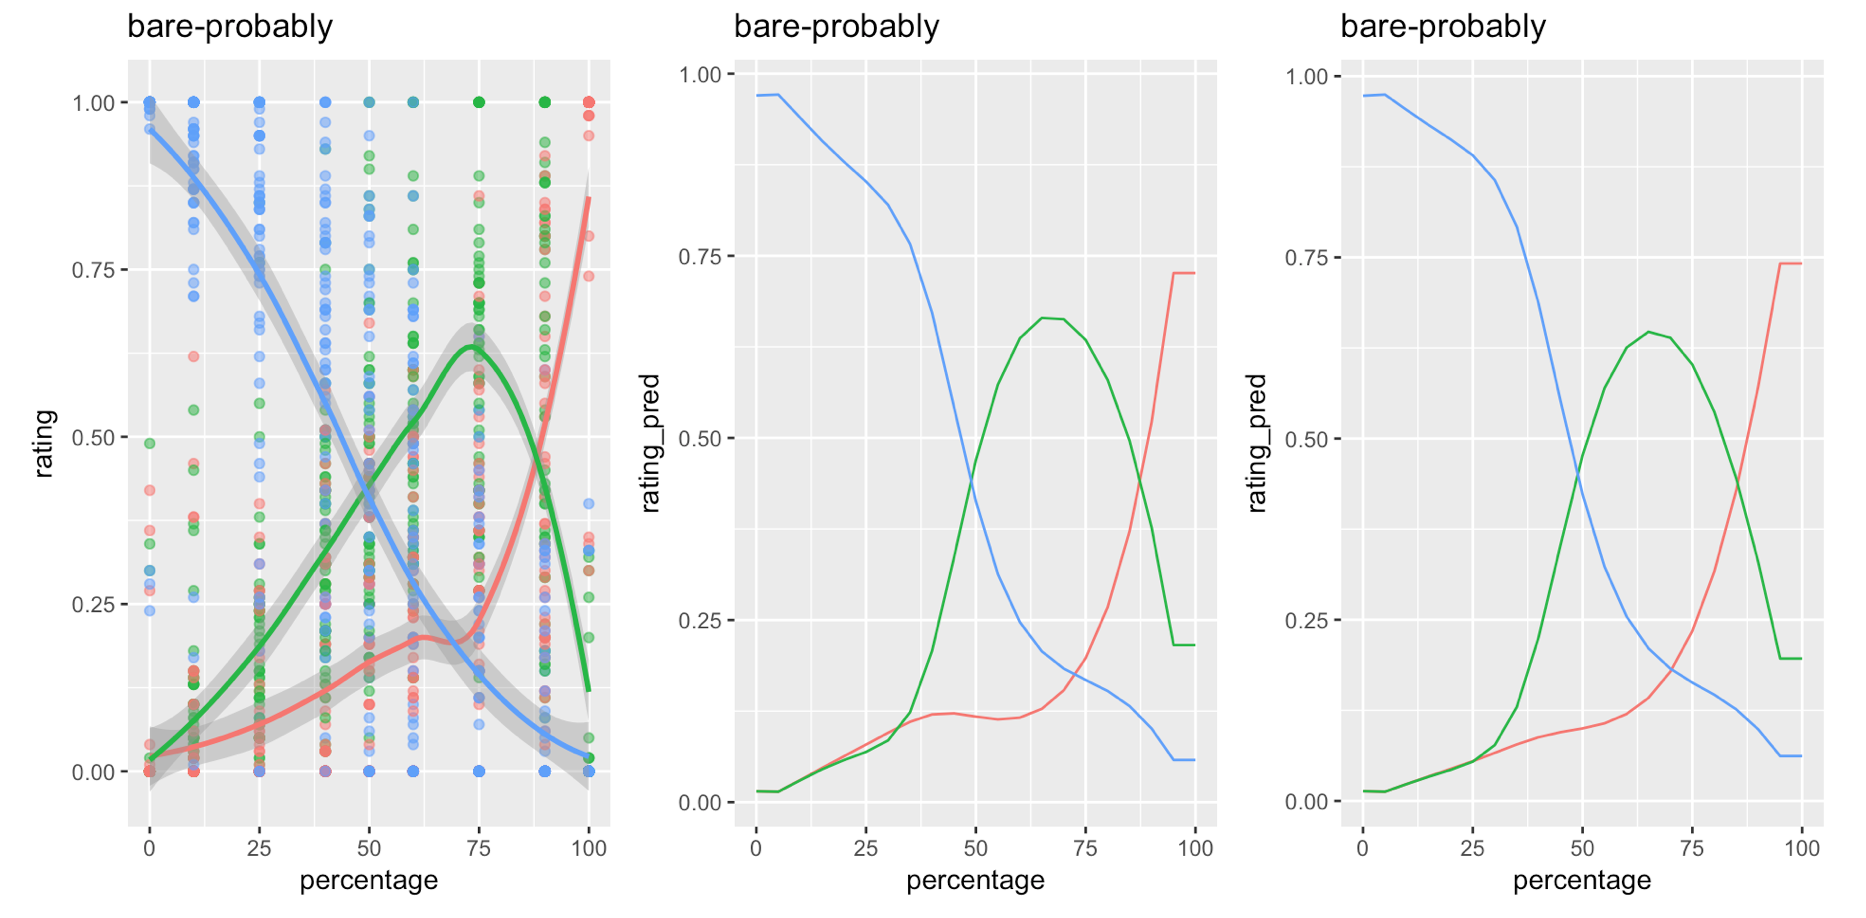
\includegraphics[width=\textwidth]{figures/bare-probably-predictions.png} \\
bare (red) - probably (green) condition

\vspace{2em}


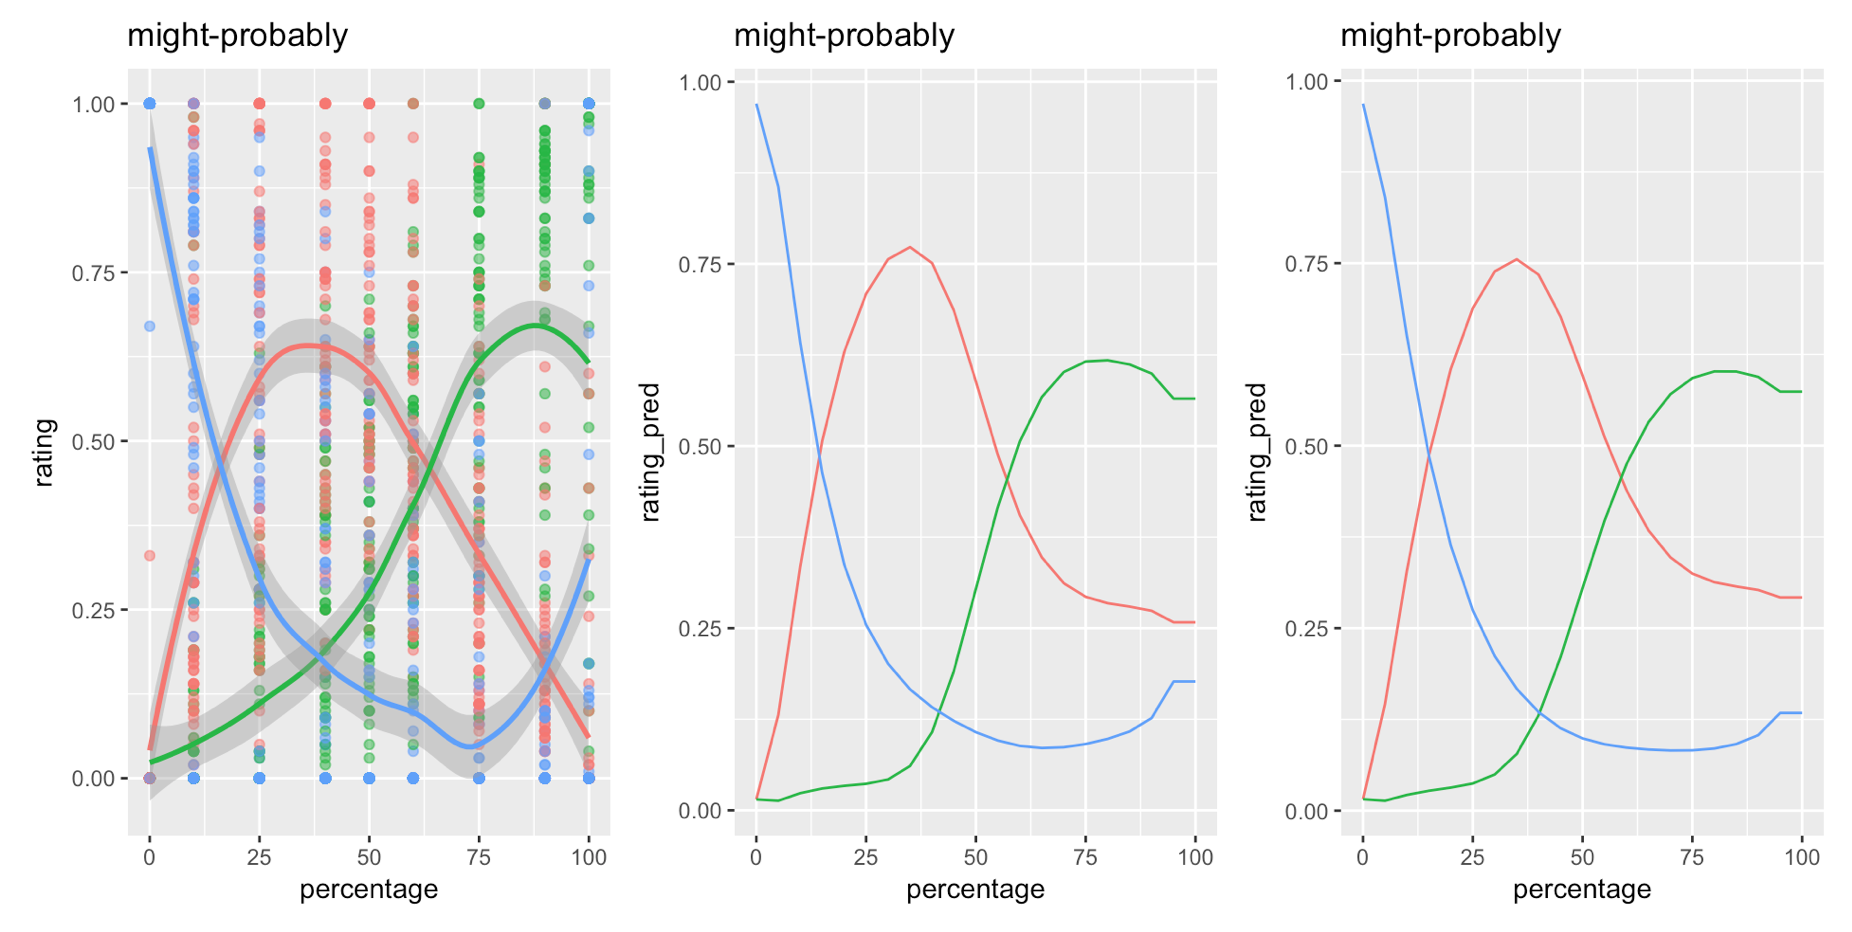
\includegraphics[width=\textwidth]{figures/might-probably-predictions.png}

might (red) - probably (green) condition

\vspace{2em}


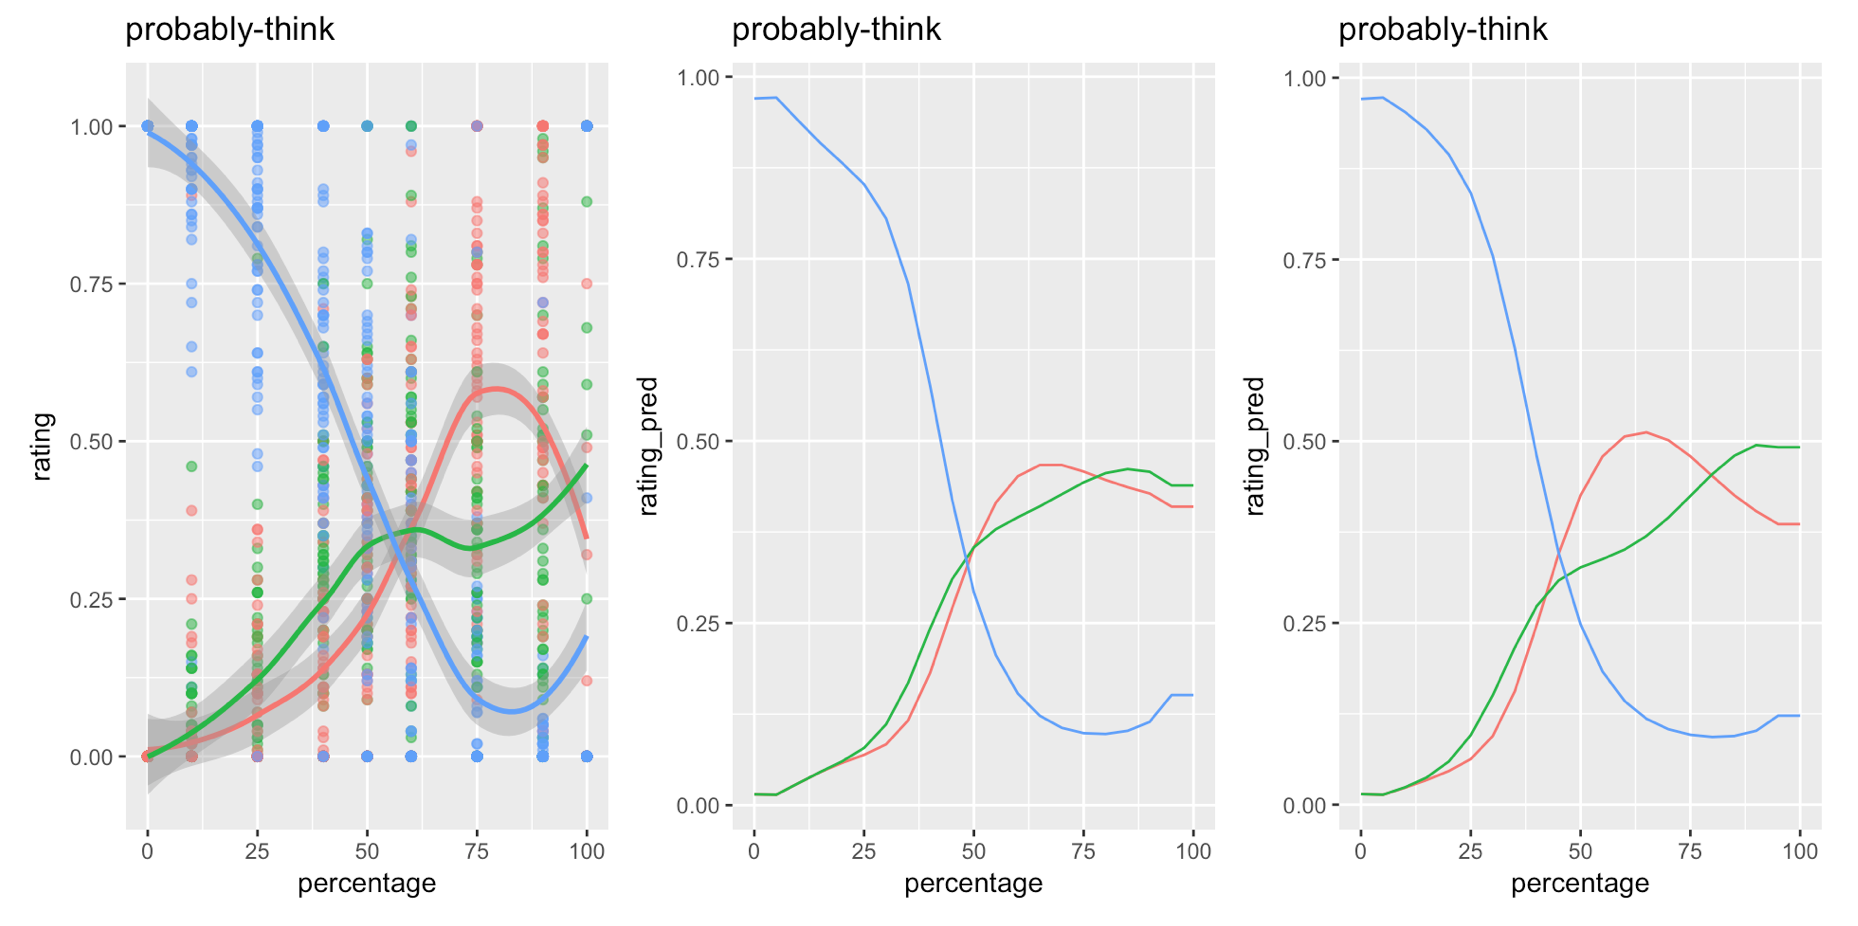
\includegraphics[width=\textwidth]{figures/probably-think-predictions.png}

probably (red) - think (green) condition

\vspace{2em}


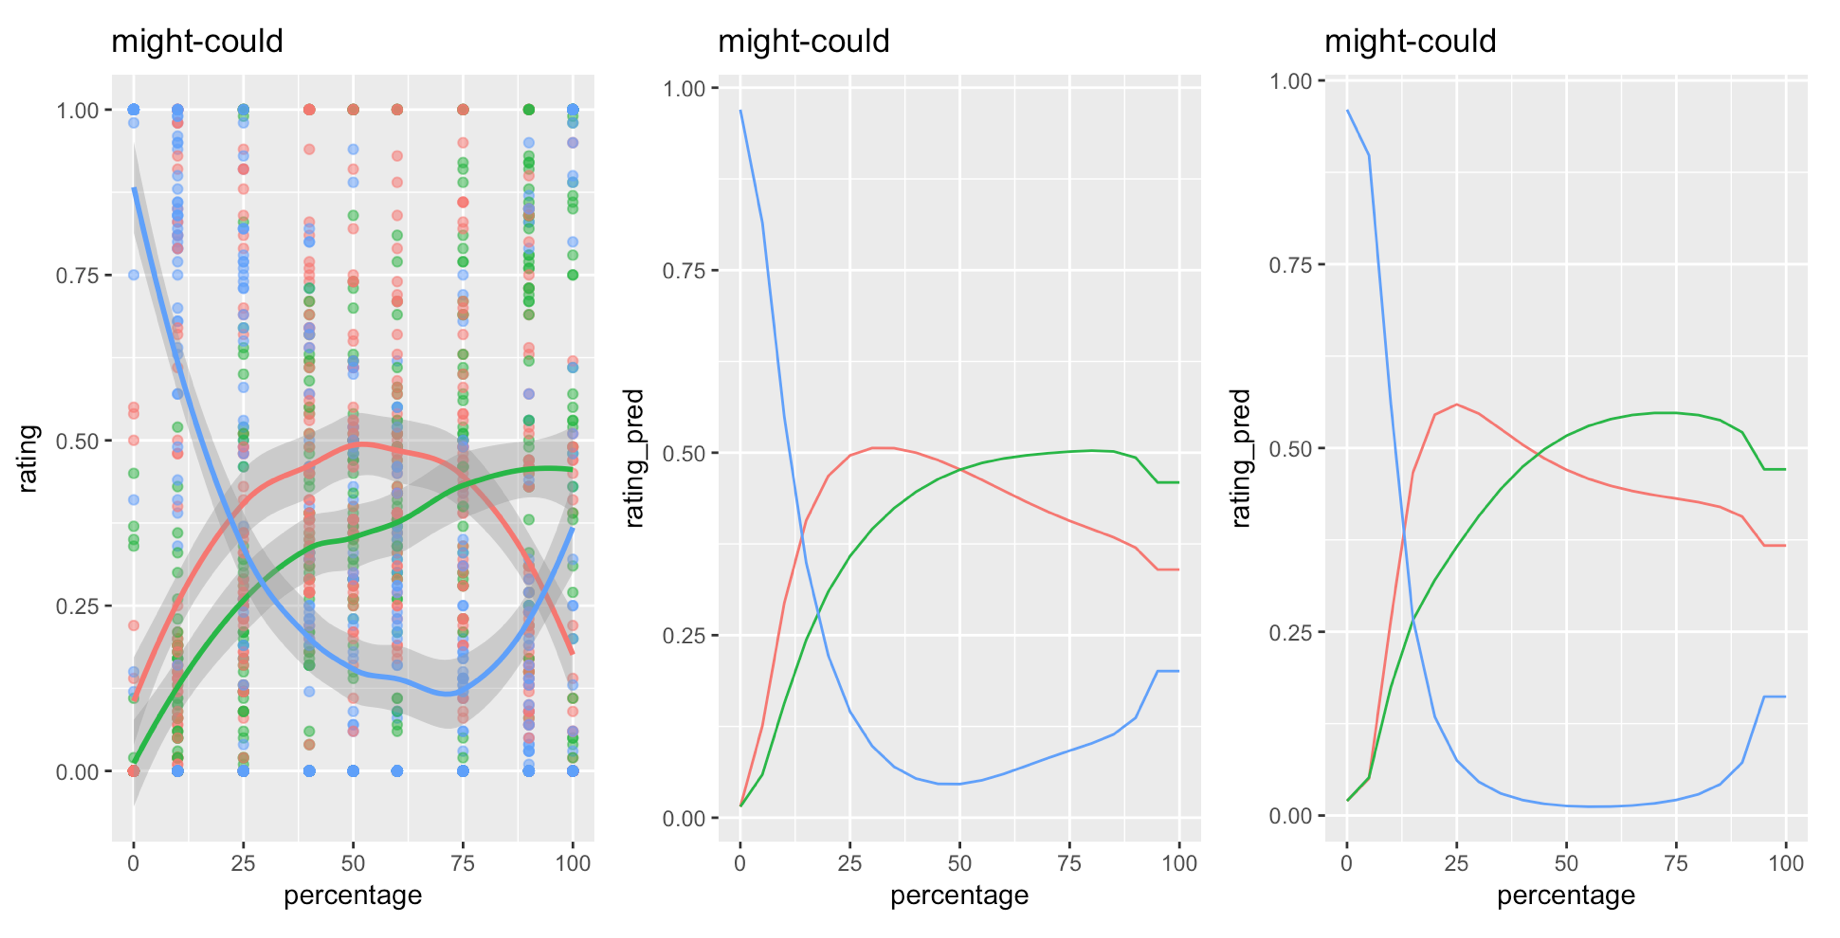
\includegraphics[width=\textwidth]{figures/might-could-predictions.png}

might (red) - could (green) condition

\vspace{2em}


\end{center}

In general, the model predicts the average participant responses very well -- in particular in cases in which there are clear contrasts between the utterances (e.g., here in the bare-might, bare-probably, and might-probably conditions). When the two utterances can be used for similar probability ranges (e.g., in the probably-think and the might-could condition), the model deviates a bit more from the experimental data (presumably because there are no clear differences between these two utterances in this context). A second issue with the model seems to be that in some conditions, participants seem to be more rational than the model estimates would suggest. For example, in the might-probably condition, the empirical ratings for \textit{probably} are higher than the predicted ratings.

We also validated our model through cross-validation. In the above figures, the right-most plot shows the model predictions if we estimate model parameters on all conditions except for the one that we are predicting. For example, the right plot for the bare-might condition shows the predictions for this condition if we estimate the parameters using the experimental data from the 14 other conditions. Overall, the predictions with the held-out training data are almost as good as the predictions of the model trained on all the data, which suggests that this is reasonable model for predicting participant's behavior.

One of the advantages of explicitly modeling participants' behavior as a Bayesian model is that we can also inspect the individual parameters, such as the distributions over thresholds $P(\theta_u)$. The following six plots show the estimated $P(\theta_u)$ for the six utterances that we included in our experiments.

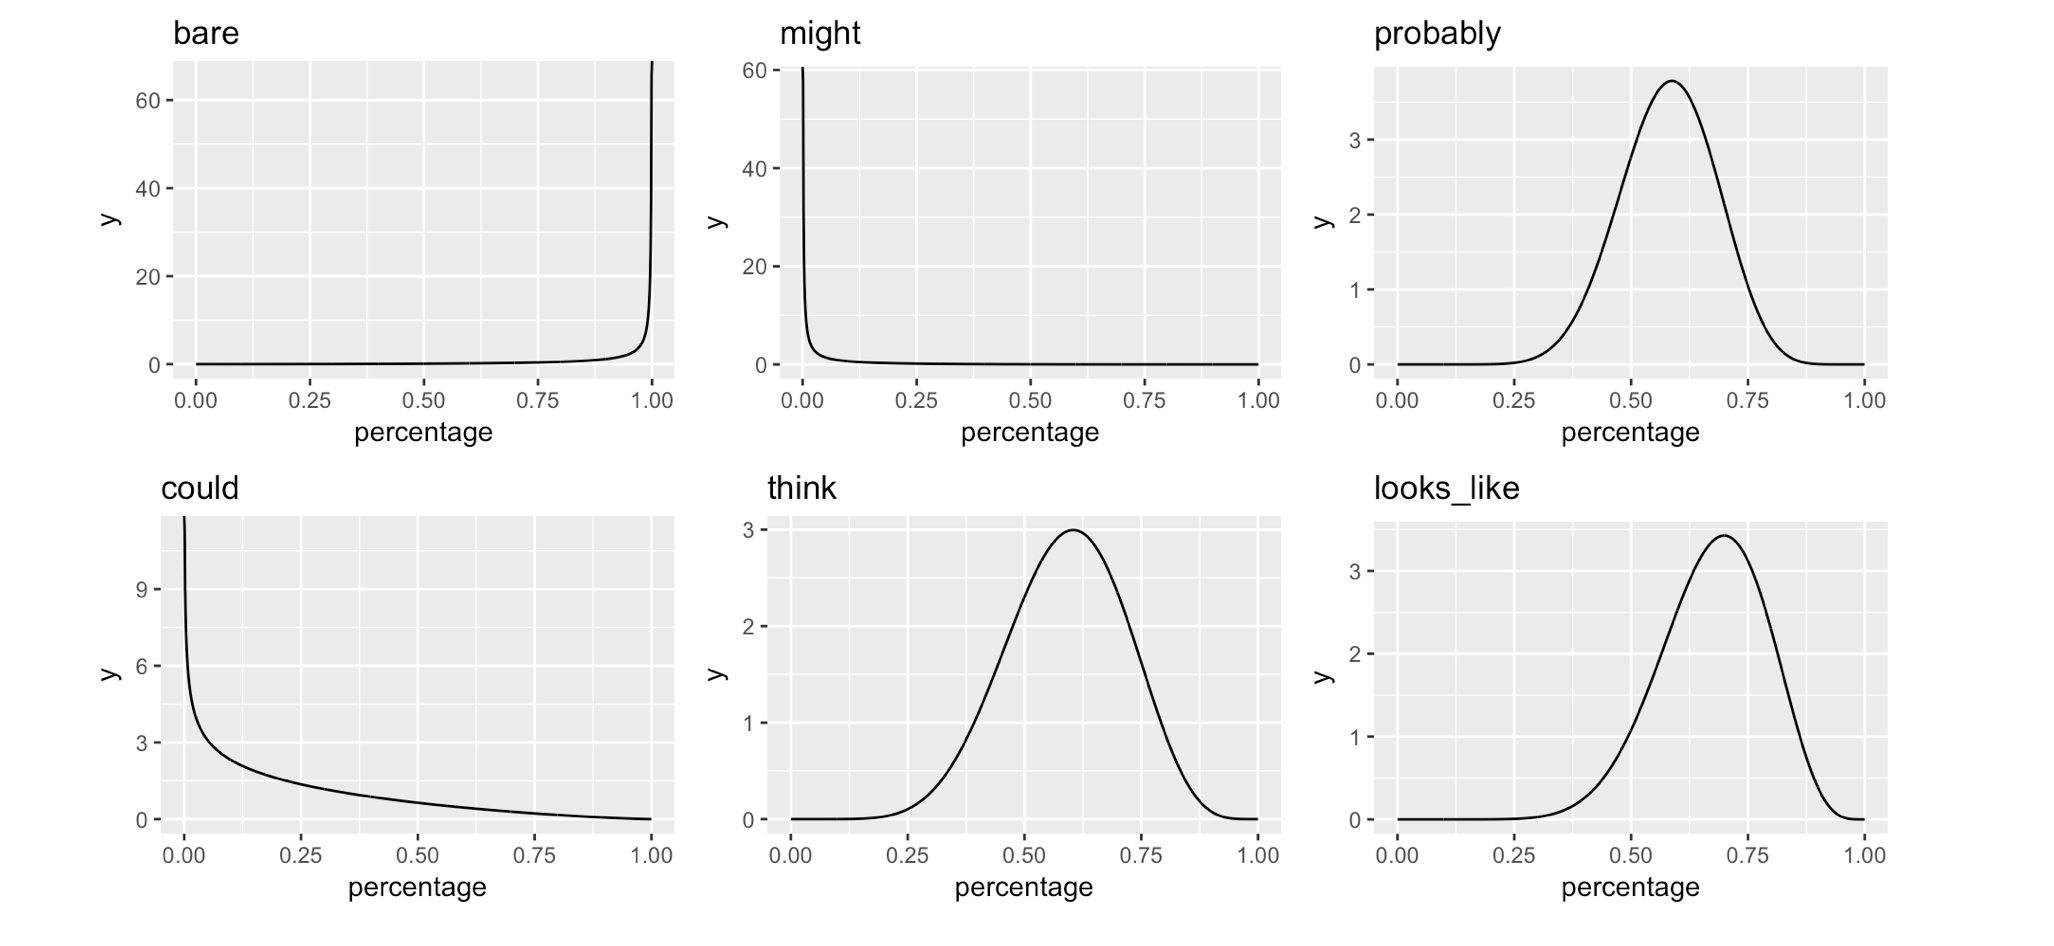
\includegraphics[width=\textwidth]{figures/threshold-distrs.png}

\vspace{2em}

Qualitatively, these estimated distributions are very much in line with semantic theories of modals (e.g., Kratzer (1991)): The  distributions for the thresholds for the possibility  modals \textit{might} and \textit{could} assign most of the probability mass to values slightly above 0; for bare statements most of the probability mass is close to 1 and for \textit{probably}, most of the probability mass is slightly above 0.5. The other two expressions, \textit{think} and \textit{looks like}, have--at least in this context--similar meanings as \textit{probably}. Furthermore, these results are also in line with recent experimental results by Pogue and Tanenhaus (submitted), who explicitly asked participants to rate how much certainty a speaker using these expressions conveyed.




\subsection{Adaptation model}

\subsubsection{Model and estimation}

We model the adaptation process as participants  a) gaining certainty about the threshold distribution that a speaker uses and b) updating the cost parameters for the individual utterances. Our main interest is in how participants update their beliefs about the thresholds for a given speaker but considering that the speaker in the exposure trials only uses \textit{might}, \textit{probably} and bare utterances, the exposure phase also suggests to participants that the speaker has a preference for these utterances over other utterances, which we can explicitly model by allowing the adaptation model to change the cost terms for different utterances. For the exposure phase, we assume that the cost of an utterance is always $c_u$ because are not presented with alternative utterances.

\vspace{1em}

\textbf{Q:} Is this a reasonable argument for/the right way of changing the cost structure during the exposure phase?

\vspace{1em}


We assume that participants are doing Bayesian belief updates when they observe utterances during the exposure trials (similarly as Qing (2014) for his model of quantifier adaptation).

\begin{align*}
P(\theta, c \mid \mathscr{D}) &\propto P(\theta, c) P(\mathscr{D} \mid c, \theta)  \\
& = P(\theta, c) \prod_{d \in \mathscr{D}} P_S(u_d \mid \phi_d; c, \theta)
\end{align*}

For the priors over thresholds $P(\theta_u)$, we take the priors that we estimated from the pre-test experimental data. For the costs, we sample from a normal distribution with $\mu=c_u$ (also estimated from the pre-test experimental data) and $\sigma=2$. The data  $\mathscr{D}$ are the 20 utterances that participants hear during the exposure phase. 

\subsubsection{Model predictions}


Participants performed the same task as in the \textit{might-probably} condition of the pre-test experiment after the exposure phase. We use the same model as in the pre-test experiment to predict participants' ratings for the utterances \textit{might} and \textit{probably} except that we are using the updated cost parameters and priors over thresholds. We use the same cost function as in the pre-test experiment, i.e., we assume that the cost for the two given utterances \textit{might} and \textit{probably} is 0.

The following plots compare the post-exposure experimental results to the predicted ratings of the model for the two adaptation conditions.


\begin{center}
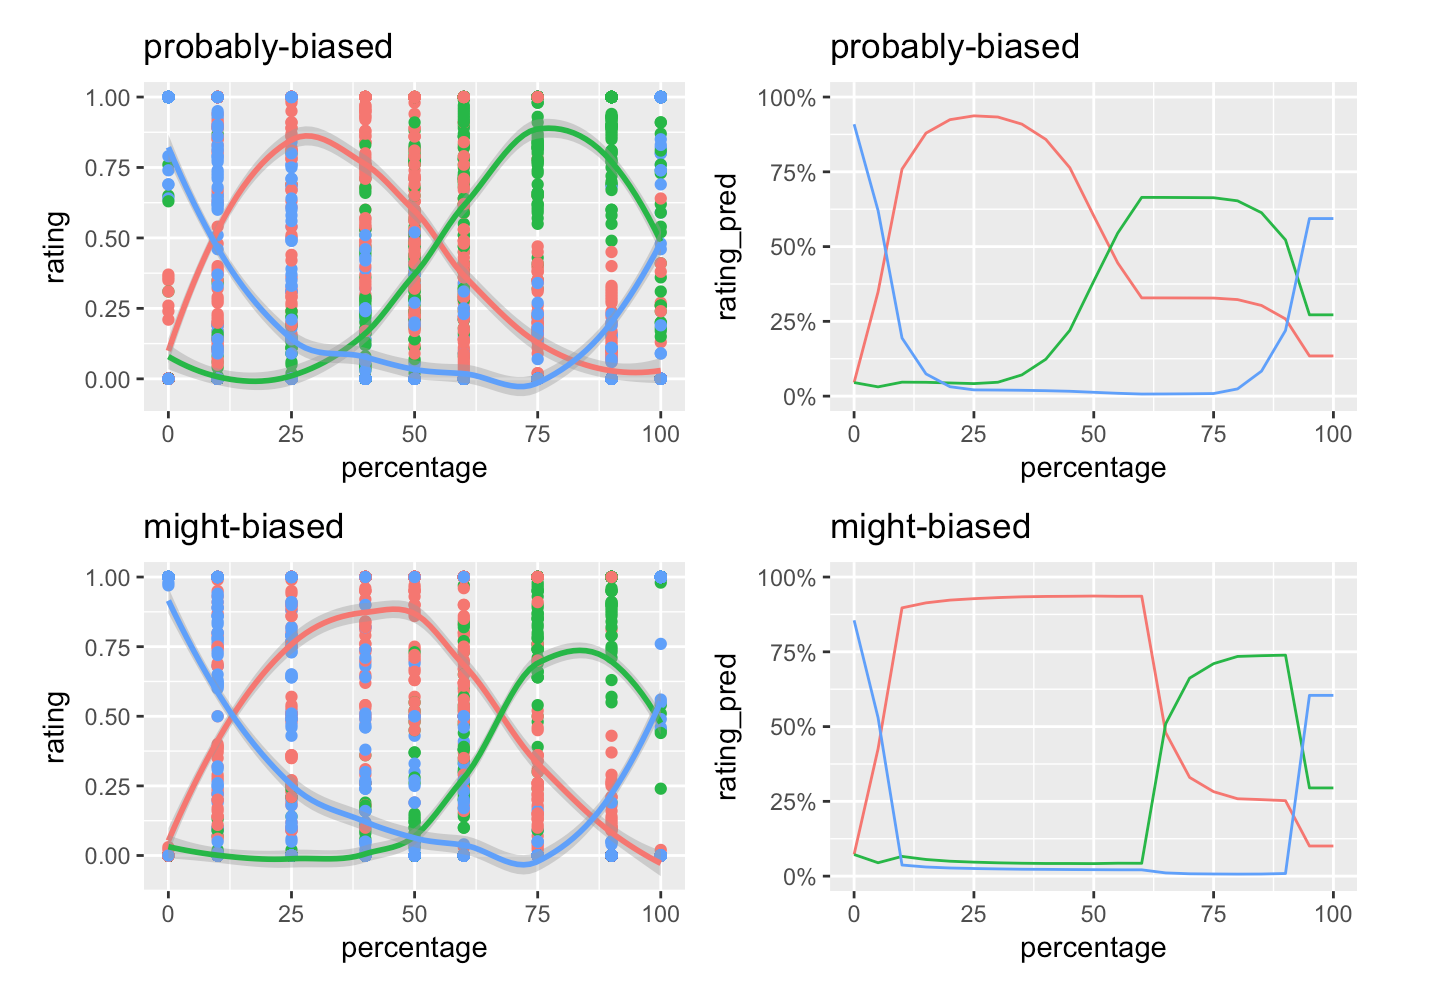
\includegraphics[width=\textwidth]{figures/adaptation-results.png}

Experimental and predicted ratings for might (red), probably (green) and other (blue) for participants in the two adaptation conditions.

\vspace{2em}
\end{center}

As these figures show, the model matches more or less the experimental results. In the probably-biased condition the model predicts that the curves cross at around 55\% of blue gumballs, which is what we observed in the data and similarly, the predicted and the actual point of intersection of the two curves in the might-biased condition are at around 65\%. However, the issue of too low ratings for \textit{probably} and the bare utterances that we already observed in the pre-test experiment, seems to be even stronger here. This effect could be lowered by increasing the rationality parameter $\lambda$ but it is not clear why people would be more rational in the adaptation experiment than they were in the pre-test experiment.

Alternatively, we could consider using a different literal listener which does not assign a uniform probability to all event probabilities $\phi$ if they are above $\theta_u$. But again, it is unclear what these distributions would look like.

As in the pre-test experiment, we can again look at the posterior distribution of $P(\theta)$ and the cost parameters for the two conditions.


\begin{center}
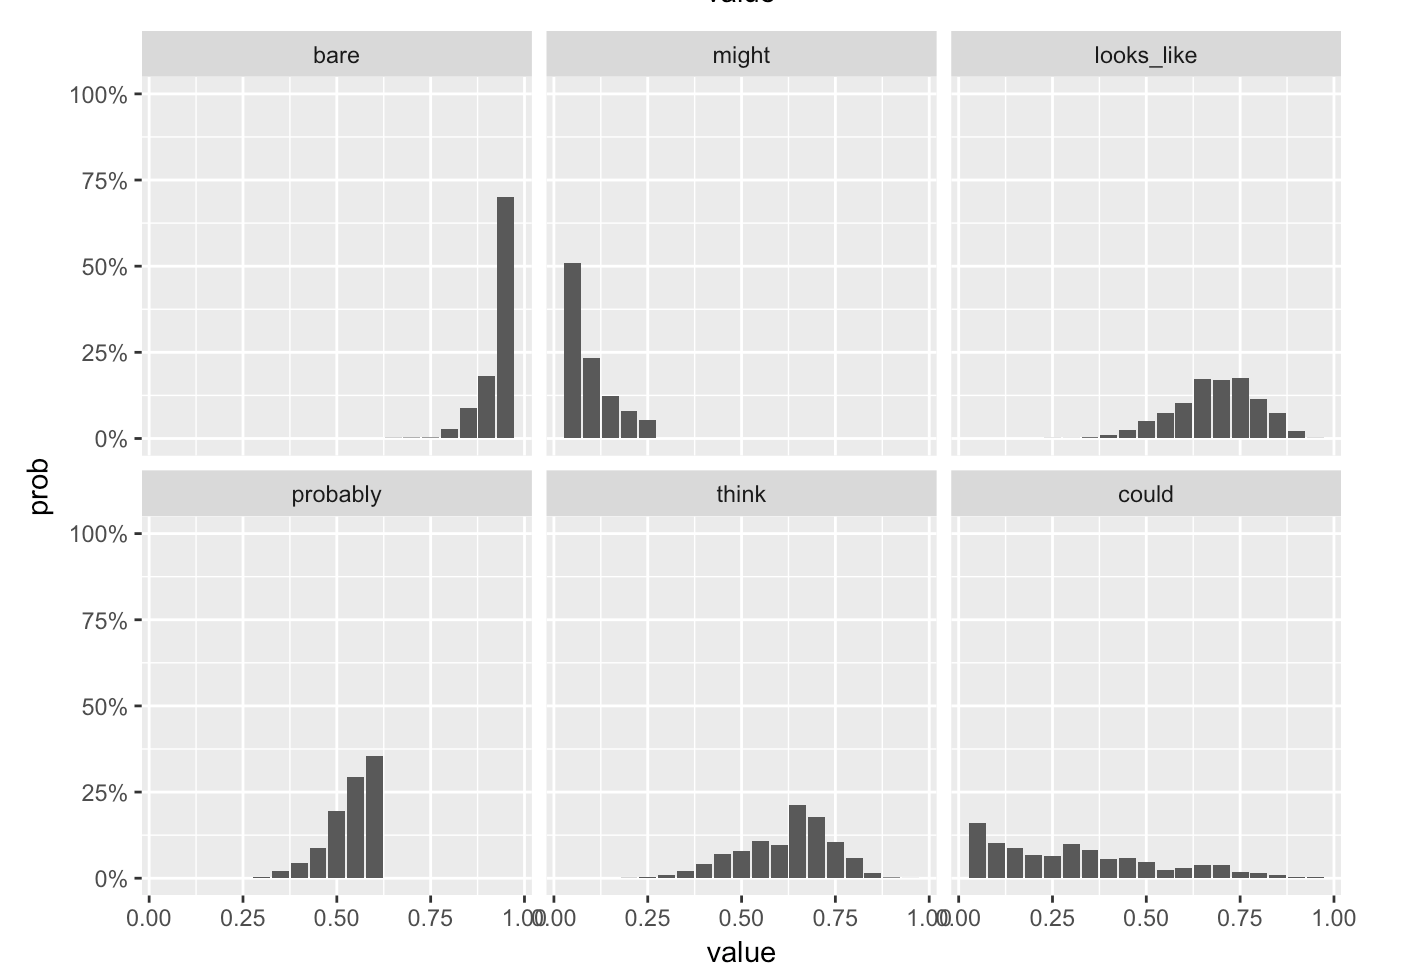
\includegraphics[width=0.9\textwidth]{figures/probably-biased-threshold-posterior.png}

Posterior distributions over threshold parameters $\theta$ in the \textbf{probably-biased} condition.
\end{center}

\begin{center}
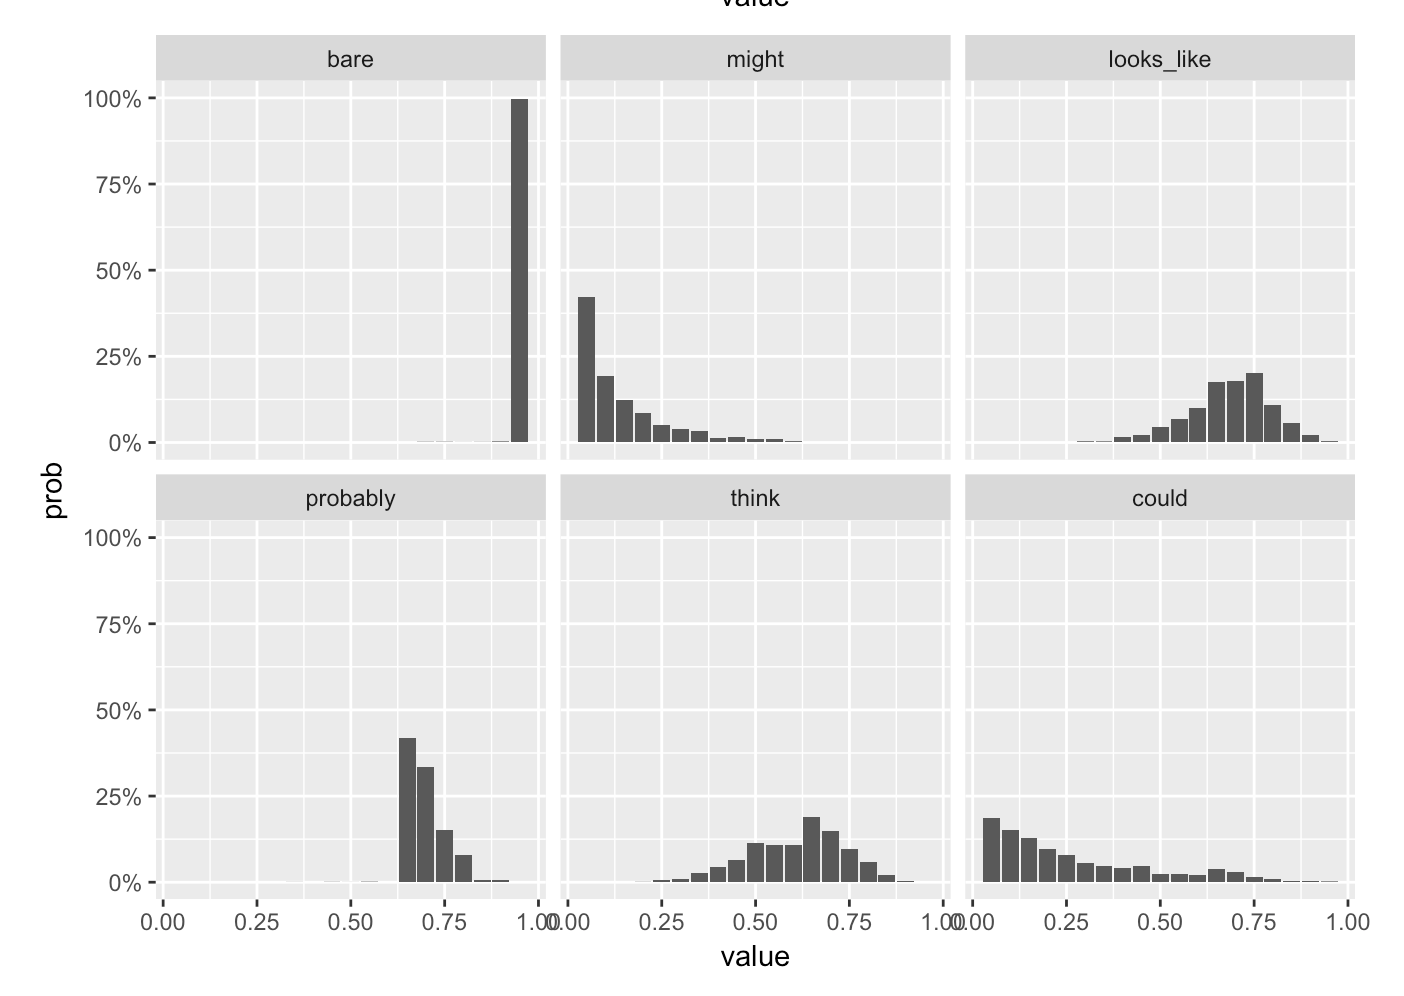
\includegraphics[width=0.9\textwidth]{figures/might-biased-threshold-posterior.png}

Posterior distributions over threshold parameters $\theta$ in the \textbf{might-biased} condition.
\vspace{2em}
\end{center}

These plots suggest that the distributions over thresholds for the three utterances that do not appear in the exposure phase remain fairly broad and match to a large extent the prior distributions.
This suggests that participants are not updating their beliefs about the use of these expressions, which is expected given that they do not see any evidence for the use of these expressions. 

\vspace{1em}
\textbf{Note:} Would be interesting to collect post-exposure ratings for e.g., the pair \textit{could} and \textit{looks like} and see if these things remain more or less unchanged.
\vspace{1em}

The distributions over thresholds for bare utterances, \textit{might} and \textit{probably}, on the other hand, differ considerably across the two conditions and are overall much narrower. In the \textit{probably-biased} condition, 
the model infers that the threshold should be at or slightly below 60\%, and the threshold for \textit{might} should be somewhere between 5 and 25\%.

In the \textit{might-biased} condition, the distribution of $\theta_{might}$ has a slightly longer tail but overall still assumes that the threshold is low.  The distribution of $\theta_{probably}$ in this condition, is shifted to the right with the most likely threshold being at 65\% and given that the speaker in this condition always uses \textit{probably} to refer to events which are 90\% likely to happen, the distribution for $\theta_{bare}$ is also shifted to the right and much narrower. 

Overall, these thresholds seem very reasonable and what is noteworthy is that the model still assigns a high probability to utterances with \textit{might} to describe events whose probability of happening is low despite the fact that participants only observe \textit{might} being used to describe  events with a probability of happening of 60\%.


\printbibliography
%\bibliography{qp-references}


%=====================================================================

%\begin{addresses}
 % \begin{address}
%    Author1 \\
%    Street \\
%    \ldots \\
%    \email{author1@email}
%  \end{address}
%  \begin{address}
 %   Author2 \\
 %   Street \\
 %   \ldots \\
 %   \email{author2@email}
 % \end{address}
 % ...
%\end{addresses}

%=====================================================================

\end{document}
